\documentclass{article}
\usepackage{listings}
\usepackage{courier}

\lstset{basicstyle=\footnotesize\ttfamily,breaklines=true}
\lstset{framextopmargin=50pt,frame=bottomline}
\usepackage{amsmath}

\usepackage{algorithm}
\usepackage[noend]{algpseudocode}

\makeatletter
\def\BState{\State\hskip-\ALG@thistlm}
\makeatother

\usepackage[letterpaper]{geometry}

\usepackage{booktabs}
\usepackage{textcomp}
\usepackage{float}
\usepackage{graphicx}
\graphicspath{{./doc_imgs/}}
\usepackage[utf8]{inputenc}

\usepackage{indentfirst}

\addtolength{\topmargin}{-1.00in}
\addtolength{\textheight}{1.5in}

\def\D{\mathrm{d}}

\begin{document}

\title{RoseLap v5: Lap Time and Point Simulation}
\author{Thaddeus Hughes (hughes.thad@gmail.com) \\ Evë Maquelin (evelyne@maquelin.com)}

\maketitle

\begin{abstract}
RoseGPE is a student design competition team at Rose-Hulman that competes in the Formula SAE competitions, typically at the Lincoln and Michigan events. RoseGPE is driven by students learning and gaining work experience, and does this by aiming to score high at competition. To do this, the team builds a new prototype vehicle every year.

The competition is historically composed of 3/8 'static' events (cost judging, design judging, business case judging) and 5/8 'dynamic' events (acceleration, skidpad, autocross, endurance, and fuel economy)- meaning there are many facets to earning points and doing well.

Lap Time Simulation can be utilized to determine the configuration of vehicle which can produce the most points at competition. Determining points outcome from the acceleration, skipad, autocross, and endurance events is largely straightforward.
\end{abstract}

\section{Problem Introduction}
Lap Time Simulation is a numerical process. The general premise is to apply simplistic physics models to a car traveling over a small, finite stretch of track with given curvature to determine the next vehicle state. By stitching these segments together, with a strategy of when to brake, shift, or otherwise drive the vehicle, the operation of a racecar under idealized conditions can be simulated with useful accuracy.

These simulation results can be useful, potentially, to assist a driver in training for a track. They can also be useful and motivating for an engineer to understand how a vehicle drives around the track in detail, monitoring grip. The real value, however, lies in the ability to vary parameters and see how they impact lap times (and fuel consumption).

These lap times can be used with point formulas and other data to determine the overall point limit of a car at a particular competition.

\section{Pre-Processing and Input Data}

\subsection{Tire Data Fitting}
As discussed in the 'Tires' section, tire models used in RoseLap v5 are rather simplistic, but are more sophisticated than the constant COF presumed in v4 and prior. To determine the four parameters, some fitting must be done.

Tire data is obtained through physical testing. We use the data purchased from the Milliken Tire Test Consortium (TTC). This contains drive-brake and combined loading, with sweeps over various conditions.

With the python tool provided in \texttt{tire\_utility}, we examine the relationship between lateral and longitudinal force as it relates to normal force.

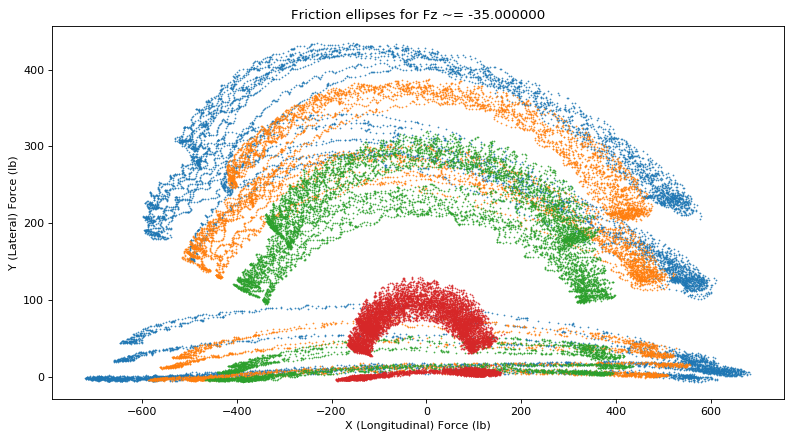
\includegraphics[width=\textwidth]{fric_ellipses.png}

The multiple colors indicate different normal forces. While imperfect, it is easy to see how fitting an ellipse to this would provide a reasonable model of tire behavior.

The first step is to determine the bins to which tire data vertical loads fall into. This is accomplished with a histogram.

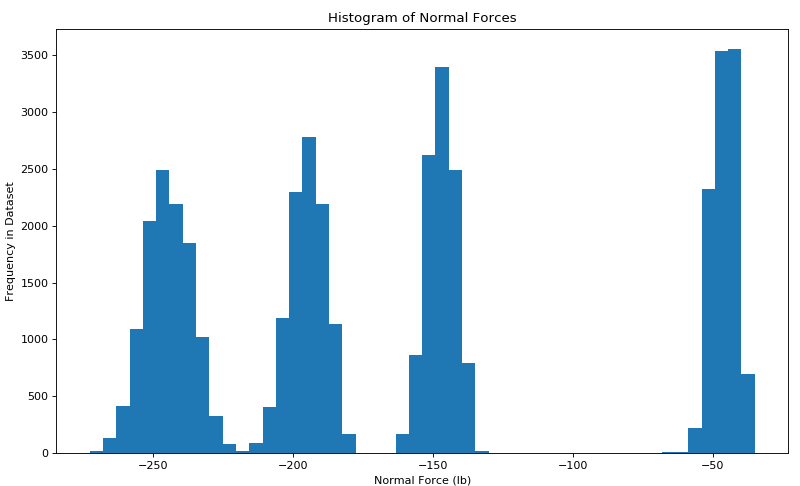
\includegraphics[width=\textwidth]{fric_hist.png}

Then, the data is analyzed in the Fz-Fx space and the Fz-Fy space. Outliers (outside of a 2-sigma confidence interval) are rejected. From here, the maximum grip datapoints from each bin are selected, and a linear regression is ran to fit these points.

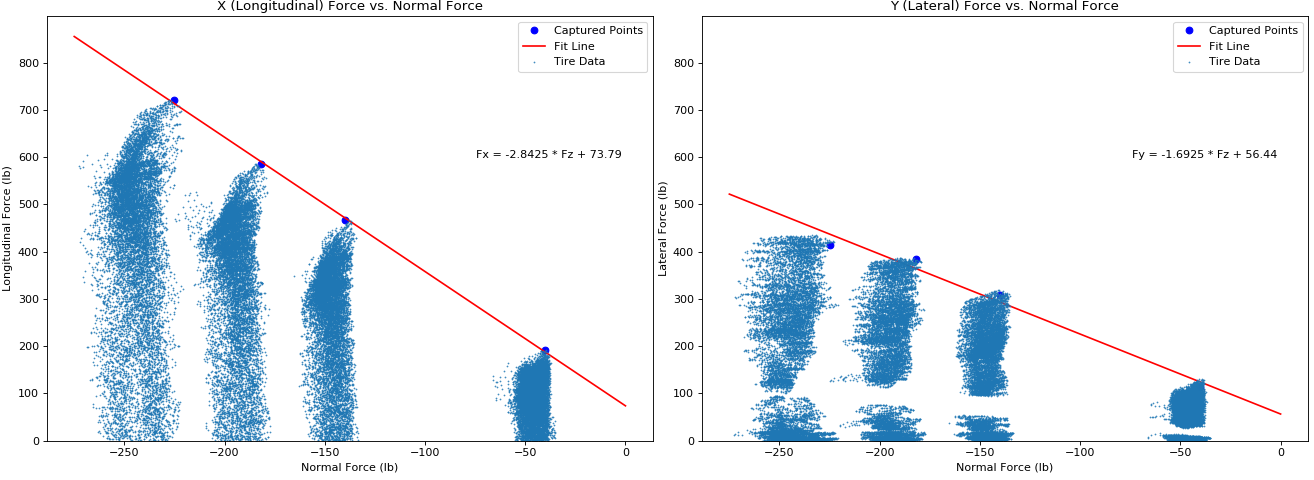
\includegraphics[width=\textwidth]{fric_regression.png}

This provides us with the four parameters for the tire: the offset and slope, in both x- and y- directions. This model is then overlaid onto the Fx-Fy data from before for comparison.

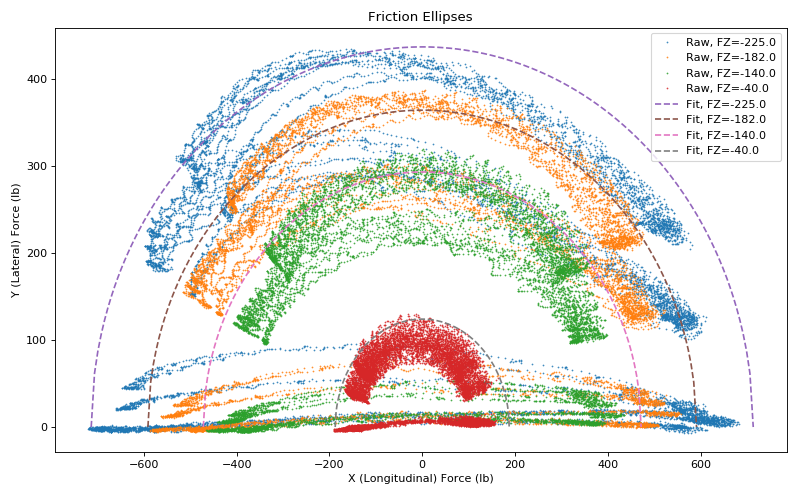
\includegraphics[width=\textwidth]{fric_ellipses_fit.png}

User adjustments can be made by changing confidence intervals, bins, or even overriding the regression results and using the charts to produce a linear fit.

\subsection{Vehicle Data Entry}

Vehicle data entry is accomplished with .YAML files. See the Example Vehicle Definition File in the Appendix.

\subsection{Tracks}

In RoseLap, tracks are sets of 'segments' analagous to an FEA mesh. A segment is parameterized as having a distance ($\Delta x$) and curvature ($k$).

Tracks may be defined in three ways:
\begin{itemize}
\item an SVG file (preferably using a spiro path)
\item a trackwalker .LOG file with a header file
\item a DXF file consisting of lines and circular arcs (NOT supported with $I_{yaw} \neq 0$)
\end{itemize}

Option 3 is becoming less supported but may come back into favor with some updates. This is because the introduction of yaw moment effects requires a track with continuous curvature; otherwise $\frac{\D k}{\D x}$ is, when numerically evaluated, effectively infinite, requiring infinite tire grip to initiate a corner.

SVG file import is accomplished with \texttt{svgpathtools}. This begins by loading all the SVG paths and computing the raw x, y, and curvature of each point at the specified mesh density. After this, a univariate spline of 2nd degree is fitted with a smoothing factor of 0.005 to the curvature data. This ensures that curvature is continuous and differentiable. The degree and smoothing parameter could be modified.

.LOG file import begins by reading a 1-line JSON file at the beginning with the following parameters:
\begin{itemize}
\item \texttt{cutoff\_start}: how many entries to cut off from the start of a track
\item \texttt{cutoff\_end}: the entry number to stop at
\item \texttt{d\_nom}: the diameter of the wheels on the trackwalker
\item \texttt{d\_scale}: the ratio of diameters between two wheels
\item \texttt{D}: the width of the trackwalker
\item \texttt{maxcurv}: a hard limit on how much curvature can be allowed
\item \texttt{smoothing}: the amount of smoothing to apply to the spline fit
\item \texttt{savgol\_amount}: the number of entries the savgol filter should average
\item \texttt{savgol\_dof}: the number of degrees of freedom to use with the savgol filter
\end{itemize}

An example of this is as follows:

\begin{lstlisting}
{"cutoff_start": 30,"cutoff_end": 1280,"d_nom": 5.74,"d_scale": 1.0185, "D": 23.0, "maxcurv": 0.15, "smoothing":0.03, "savgol_amt":351, "savgol_dof":2}
0,0
15,4
26,11
36,22
50,36
...
\end{lstlisting}

The trackwalker log is then processed to determine distance, curvature, and cartesian coordinates for all points on the track.
\begin{align}
	\Delta l_{i} = 2 (l_{1,i}-l_{1,i-1}-l_{2,i}+l_{2,i-1})\\
	d_i = \frac{l_{1,i}-l_{1,i-1} + l_{2,i} - l_{2,i-1}}{2}\\
	k_i = \frac{\Delta l_i}{D d_i}\\
	\theta_i = theta_{i-1} + d_i k_i\\
	x_i = x_{i-1} + \sin(\theta_i) d_i
	y_i = y_{i-1} + \cos(\theta_i) d_i
	l_i = l_{i-1} + d_i
\end{align}

The most important data is in the $l$, $d$, and $k$ vectors. Any element in $k$ greater in absolute value than \texttt{maxcurv} will be truncated to $\pm$ \texttt{maxcurv}. The $k$ vector is passed through a savgol filter with the specified degrees of freedom and smoothing. This removes most of the noise but still leaves a curvature profile that is rough and jagged. This filtered data is then passed through a univariate spline with 5 degrees of freedom and the specified amount of smoothing.

Visually, this looks as follows:

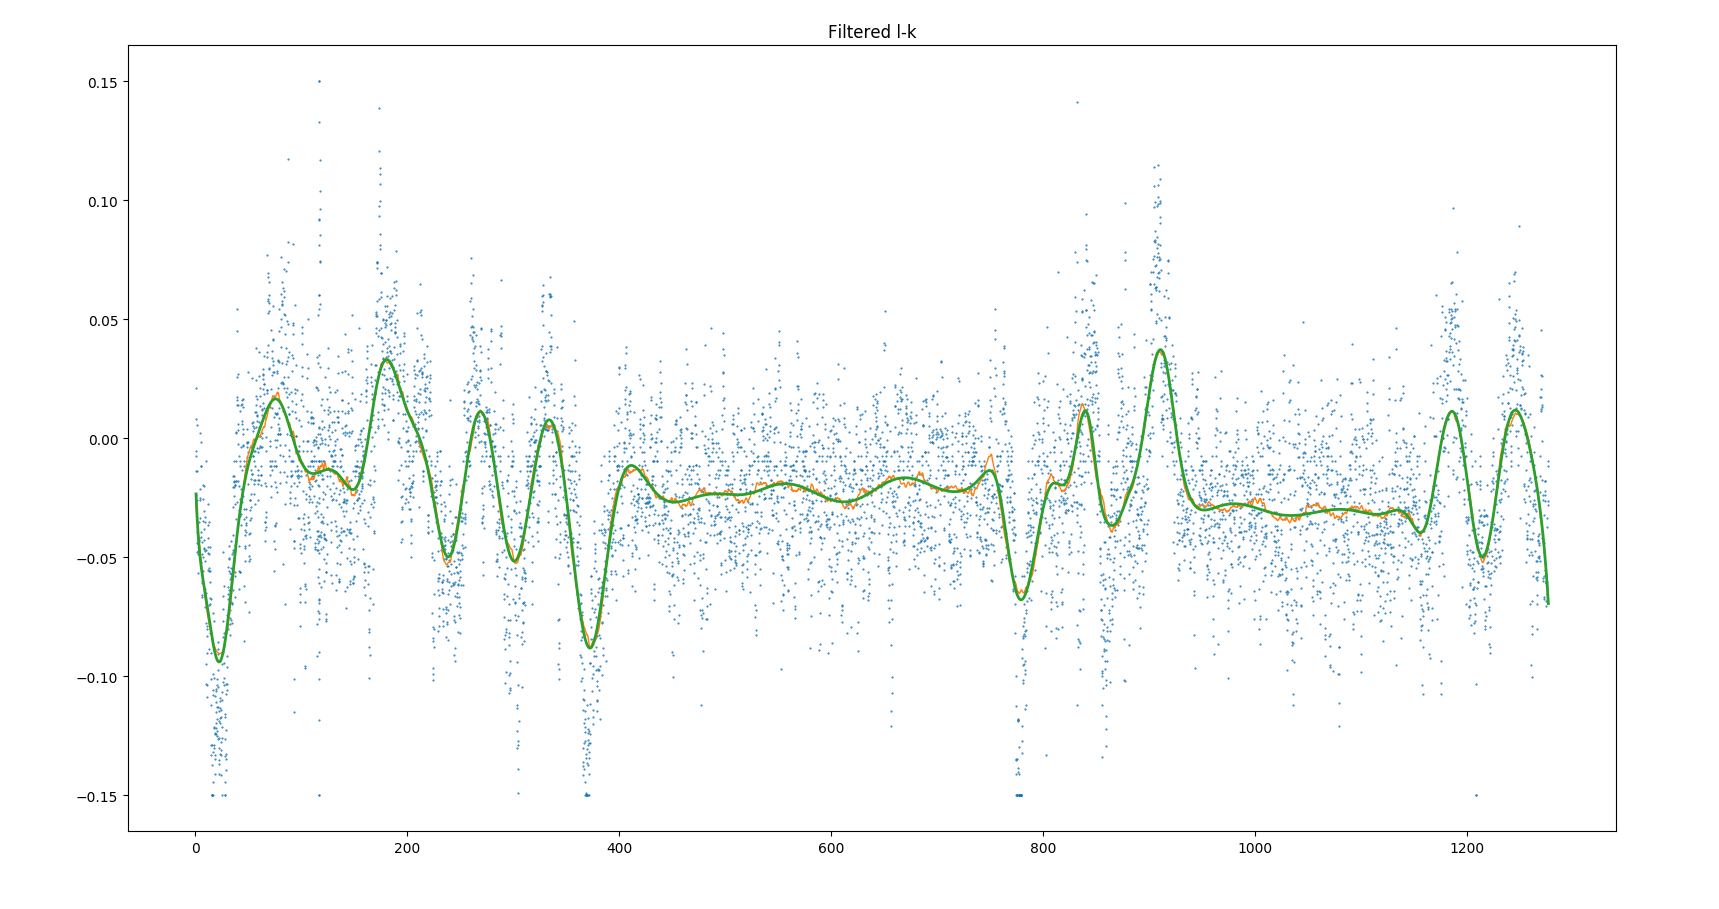
\includegraphics[width=\textwidth]{tw_filtering.png}

the unfiltered $k$ vector is the blue dots, the filtered data is the orange line, and the smoothed data is the green curve.

The fitting process is done at runtime, but the track can be previewed by using \texttt{input\_processing.py} as a command-line tool so that the fitting parameters may be adjusted. Usage: \texttt{input\_processing.py path/to/logfile.log <segment size>}

\section{Component Models}

\subsection{Tires}

Tire models are extremely complicated if they are to be accurate- but this complexity can be a distraction from the major characteristics of tires that concern us. This behavior is that tires do not have a constant coefficient of friction- it decreases with additional normal force. Alternatively, we can model the tires as having some baseline, or 'offset' grip at zero normal force, and as normal force increases, maximum grip increases linearly.

\begin{center}
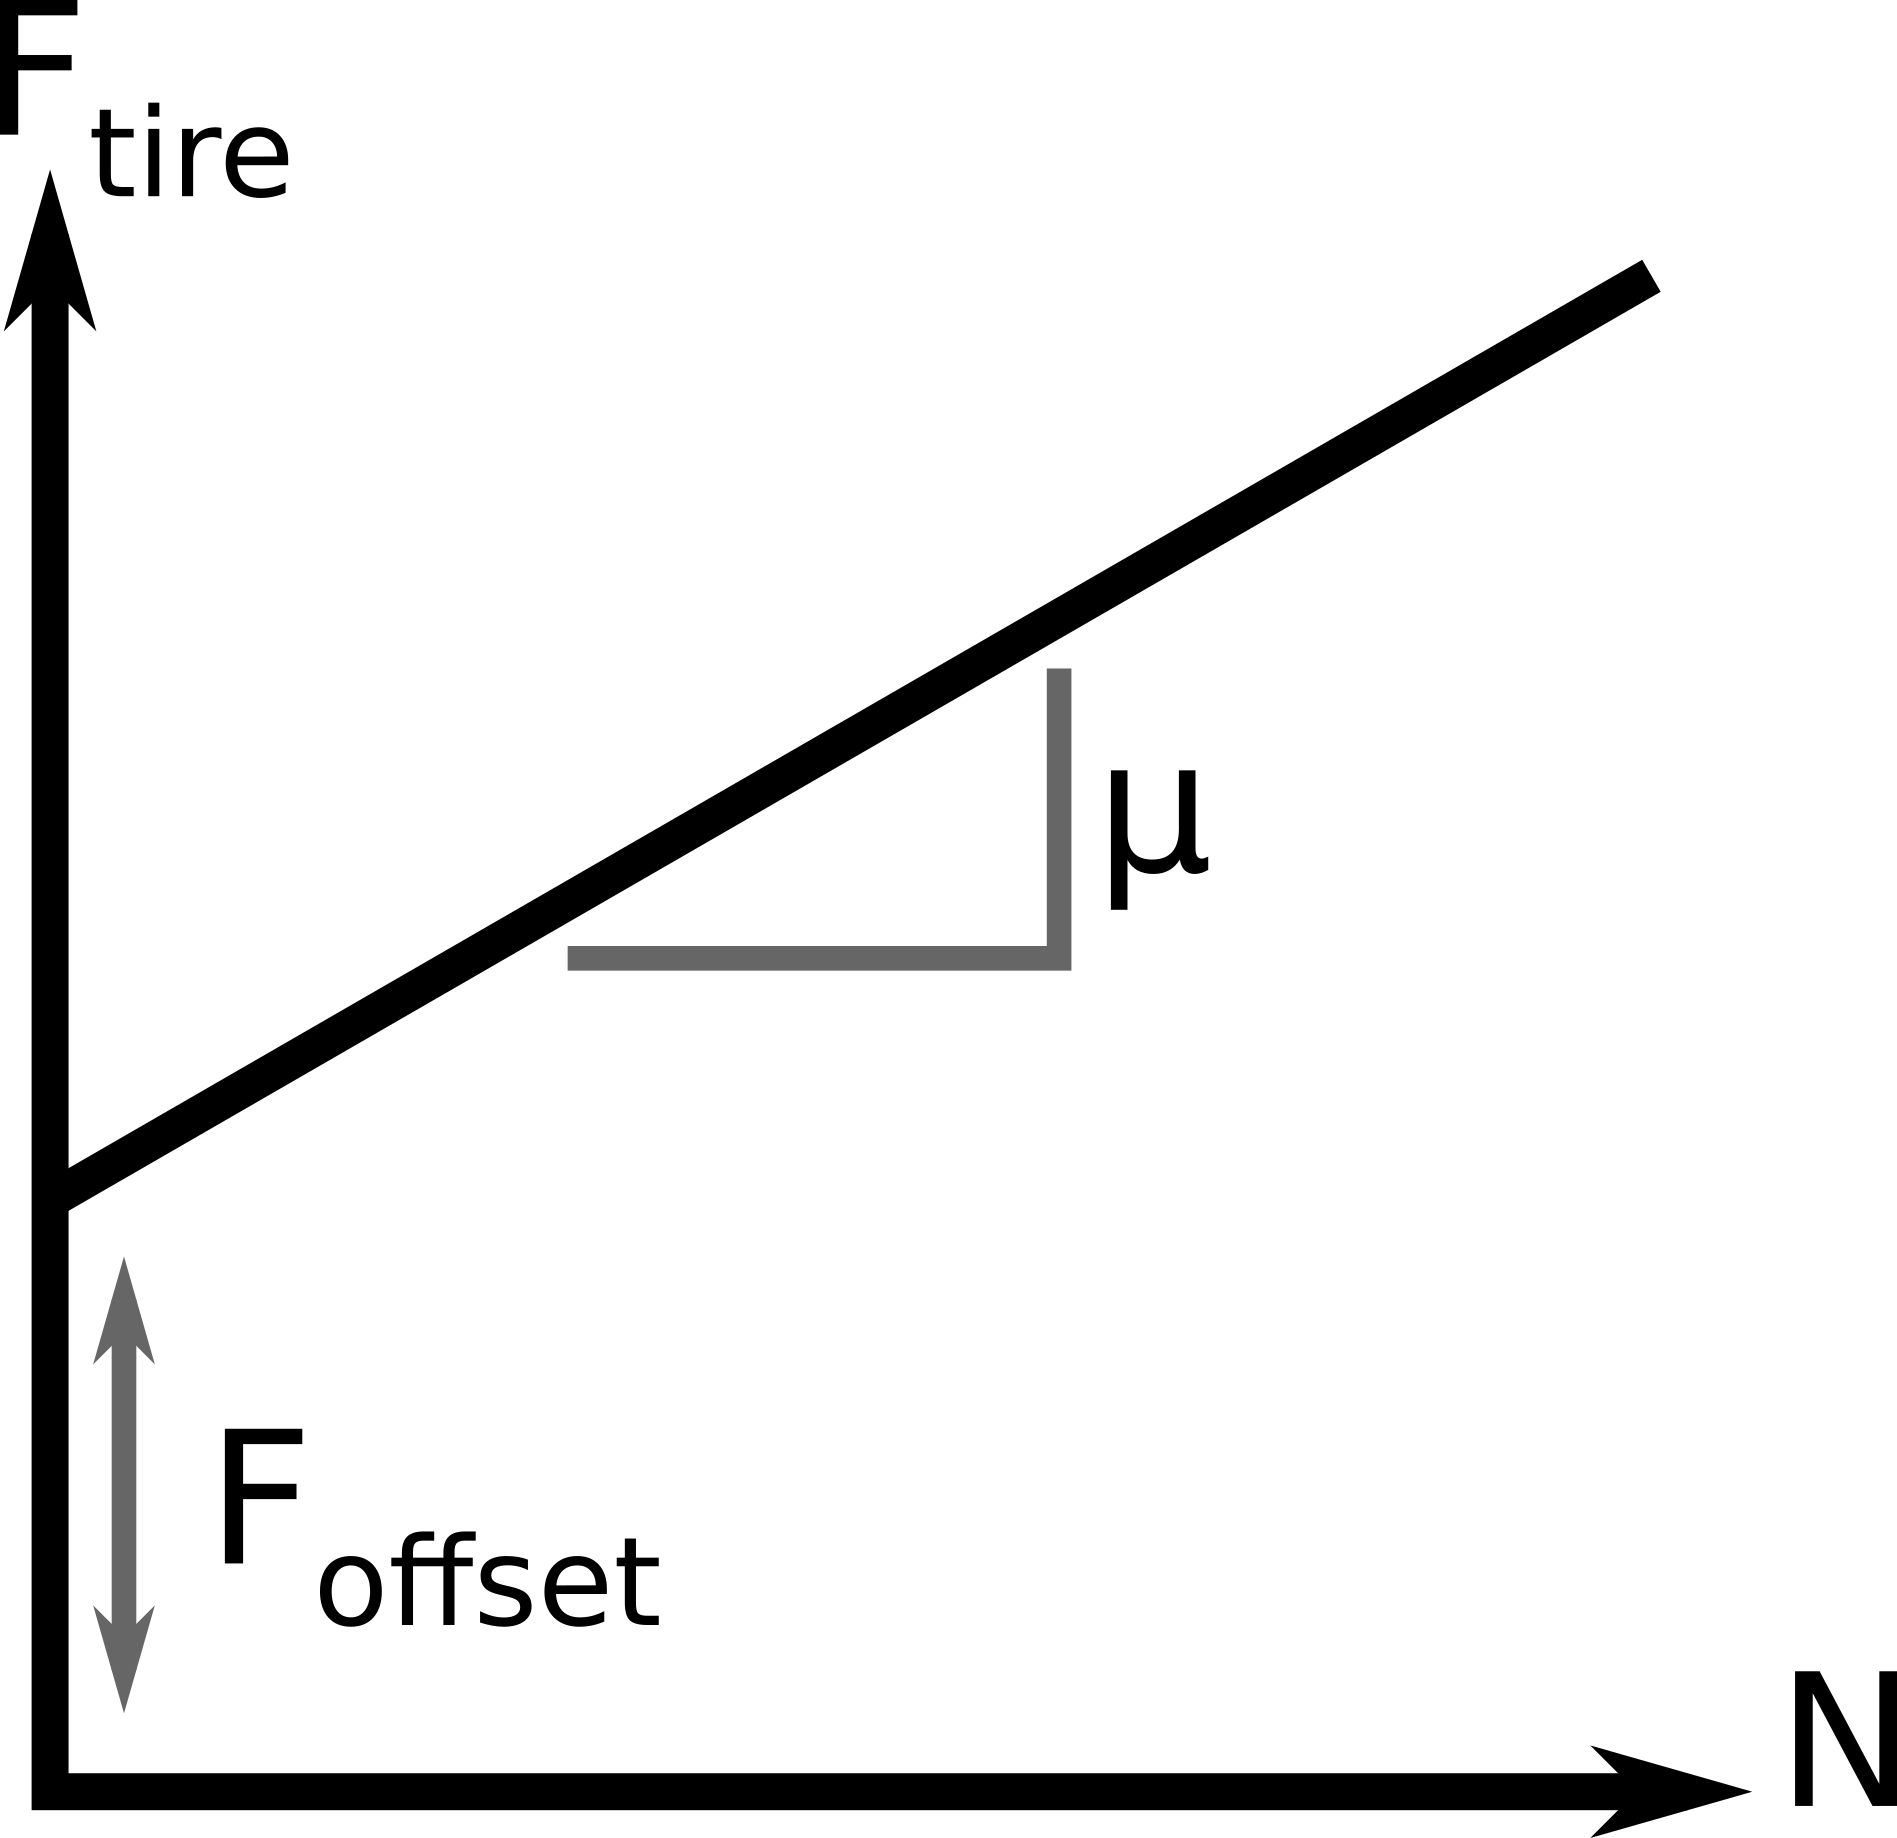
\includegraphics[height=0.3\textwidth]{tire_line.png}
\end{center}

\begin{align}
	F_{tire,max,lat} = F_{tire,offset,lat} + \mu_{tire,lat} N \\
	F_{tire,max,long} = F_{tire,offset,long} + \mu_{tire,long} N
\end{align}

The parameters here are only for one tire. If we wish to look at the lumped characteristics of multiple tires, we will need to do some simple division, and at the end of it all, multiply by the number of tires.

\begin{align}
	F_{tire,max,lat} = F_{tire,offset,lat} + \mu_{tire,lat} \frac{N}{n_{tires}} \\
	F_{tire,max,long} = F_{tire,offset,long} + \mu_{tire,long} \frac{N}{n_{tires}}
\end{align}

The parameters ($\mu$ and $F_{tire,offset}$) can be found from experimental tire data for various tires. The easiest method is to find lines that meet the outer capabilities of the tires, which will be at optimal operating conditions (camber, toe, slip rate, slip angle, and temperature).

Of course, a racecar tire is rarely purely in one of these conditions- we must determine the limits in a multi-axis loading. At a given normal force, a 'friction ellipse' can be produced that intercepts these limits.

\begin{center}
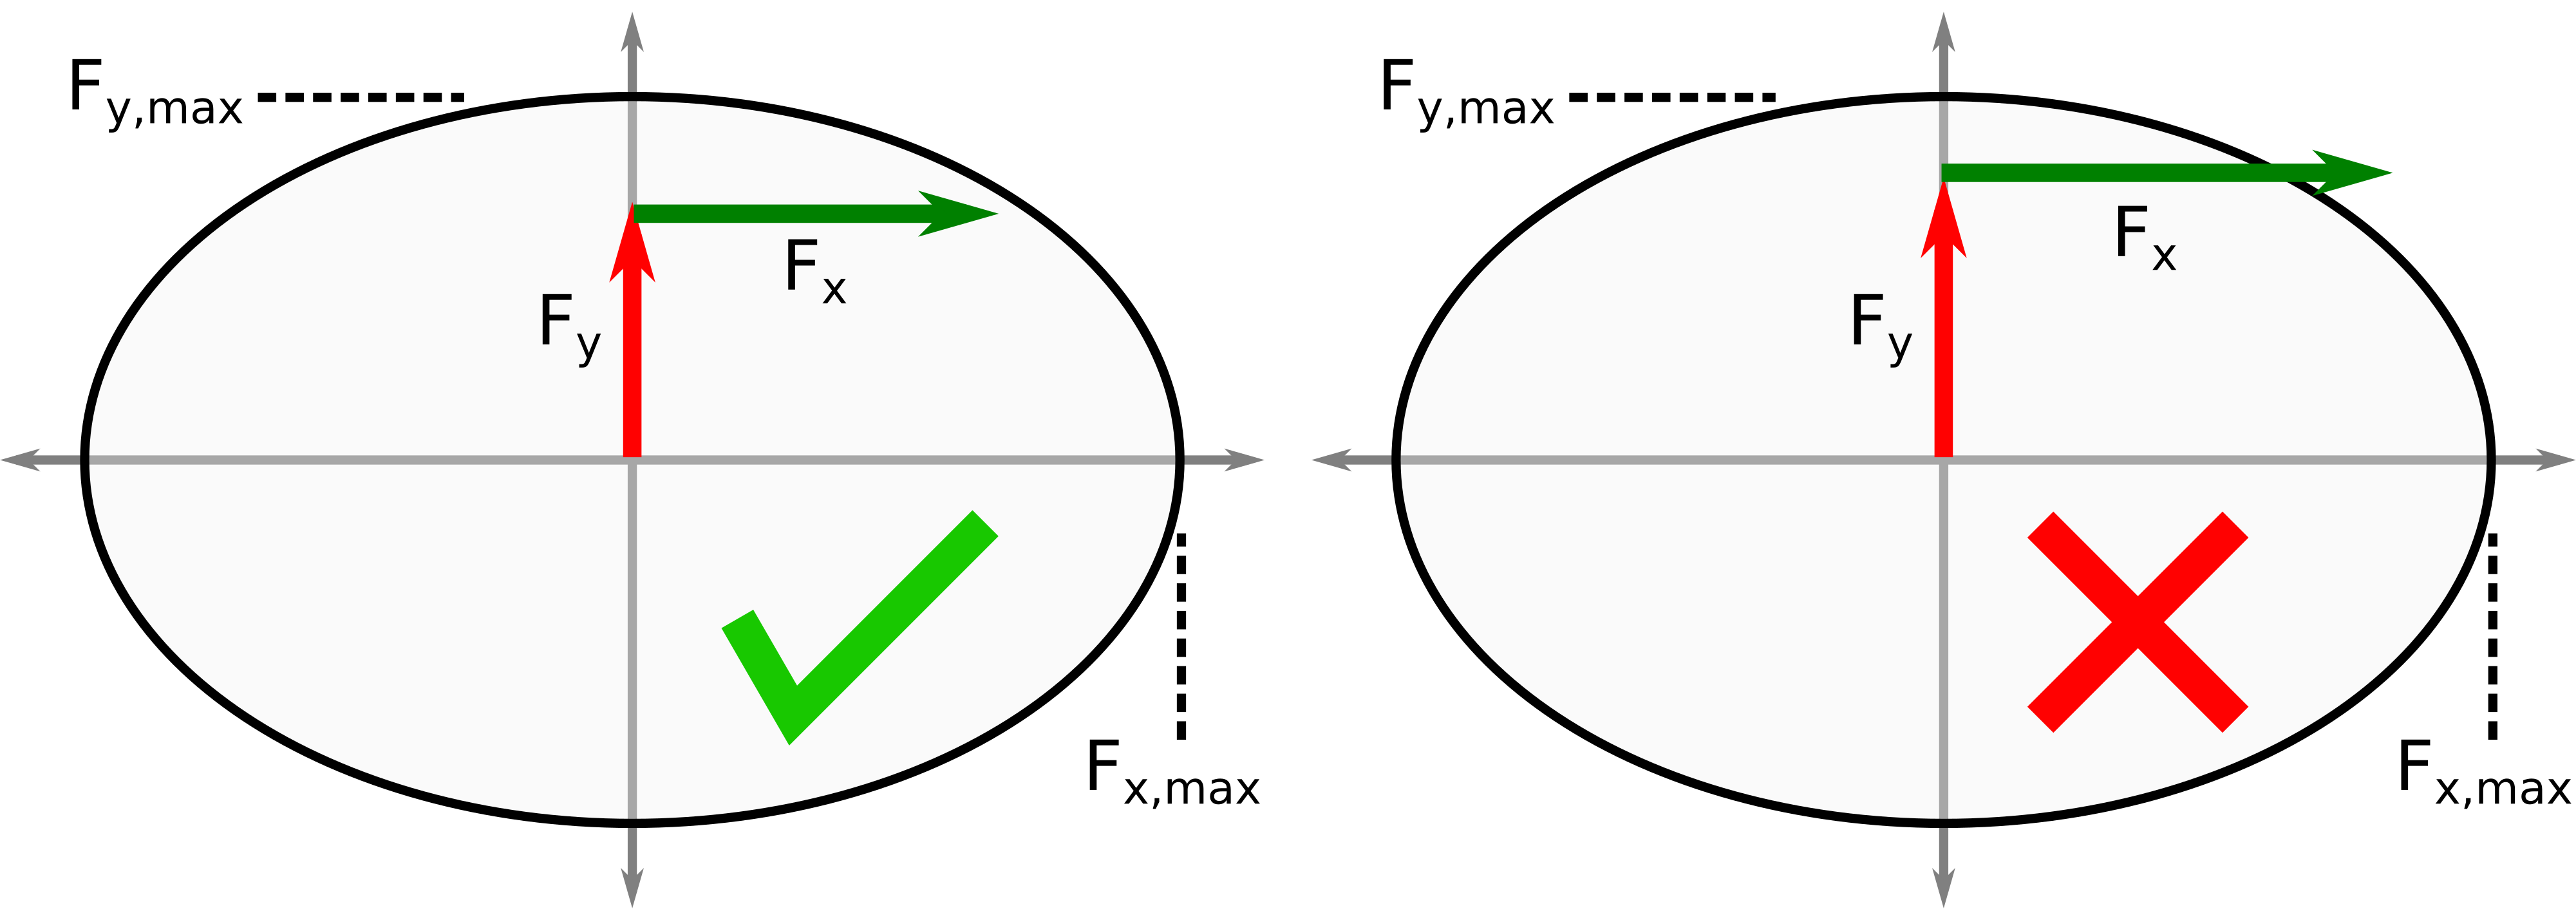
\includegraphics[width=\textwidth]{tire_ellipse.png}
\end{center}

This can be written as

\begin{align}
	\frac{F_{tire,lat}^2}{F_{tire,max,lat}^2} + \frac{F_{tire,long}^2}{F_{tire,max,long}^2} <= 1
\end{align}

We can solve, then, for the 'remaining' lateral or longitudinal force that the tire can apply before slipping (this is still for one tire, but the lateral force is for the vehicle as a whole).

\begin{align}
	F_{tire,remaining,long} = F_{tire,max,long} \sqrt{1-(\frac{F_{tire,lateral}}{n_{tires} F_{tire,max,lat}})^2} 
\end{align}

\subsection{Aerodynamics}

Aerodynamic forces on the vehicle obey a square law relationship:

\begin{align}
	F_{down} = \alpha_{down} v^2, \\
	F_{drag} = \alpha_{down} v^2, \\
\end{align}

where $\alpha$'s are scaling constants computed from the aerodynamic forces at 35 miles per hour:

\begin{align}
	\alpha = \frac{F_{35 MPH}}{(35 MPH)^2}
\end{align}

The drag and downforce can be defined for three different aerodynamic 'modes': Full, Drag-Reduced (acceleration), and Airbrake (braking).

\subsection{Powertrain}

The force developed by the powertrain at the tires is modeled as a function of vehicle velocity and current gear.

\begin{align}
	\omega_{crank} = \frac{v}{r_{tire}} N_{final} N_{transmission,i_{gear}}, \\
	F_{long,engine,limit} = T_{engine}(\omega_{crank}) N_{final} N_{transmission,i_{gear}},
\end{align}

Where $N$ is a gear ratio, $i_{gear}$ is the gear number, and $\omega_{crank}$ is the angular velocity of the crankshaft. $T_{engine}$ is a linear interpolation representing the torque curve of the engine. For velocities that cause the engine to hit its 'rev limiter', the engine is modeled as producing zero power. For velocities that are below the lowest datapoint specified in the torque curve, the engine is modeled as producing the torque at the lowest specified RPM.

It takes a finite amount of time, $t_{shift}$ in order for a shift to occur. During this time, the powertrain produces no power. Another gear is chosen with a different gear than the currently selected one will yield a higher $F_{tire}$. When this happens, the driver shifts in the direction of this gear (the transmission is sequential, not fully manual). When the vehicle brakes, the gear is 'reset', and when the powertrain is used again, the best available gear is used, regardless of what was engaged prior.

% FIXME: Efficiency (C02)

\subsection{Driver}

The driver we assume (with some noted exceptions) is one which seeks to follow the ideal that racing is about maximizing acceleration in the correct direction. They use all available tire grip or engine power whenever possible, and brake as late and hard as possible. This driver does not exist in reality, but is a useful model allowing us to push the bounds for what the car can be driven to.

\subsection{Code Implementation}
These physics which are reused throughout different overall vehicle models are implemented in \texttt{vehicle.py}, which defines the \texttt{Vehicle} object type which contains methods to access this physics and has the attributes of the vehicle. Explanation of implementation is relatively straightforward and is left to the documentation in this file.

\section{Single-Tire, Point-Mass Model}

\subsection{Physics}

The physics behind a racecar are rather complicated. However, they can be simplified with the point mass assumption. This is the assumption that the car acts as a single point where all loads are applied, with no suspension to complicate tire grip and steering or tire characteristics.

\begin{center}
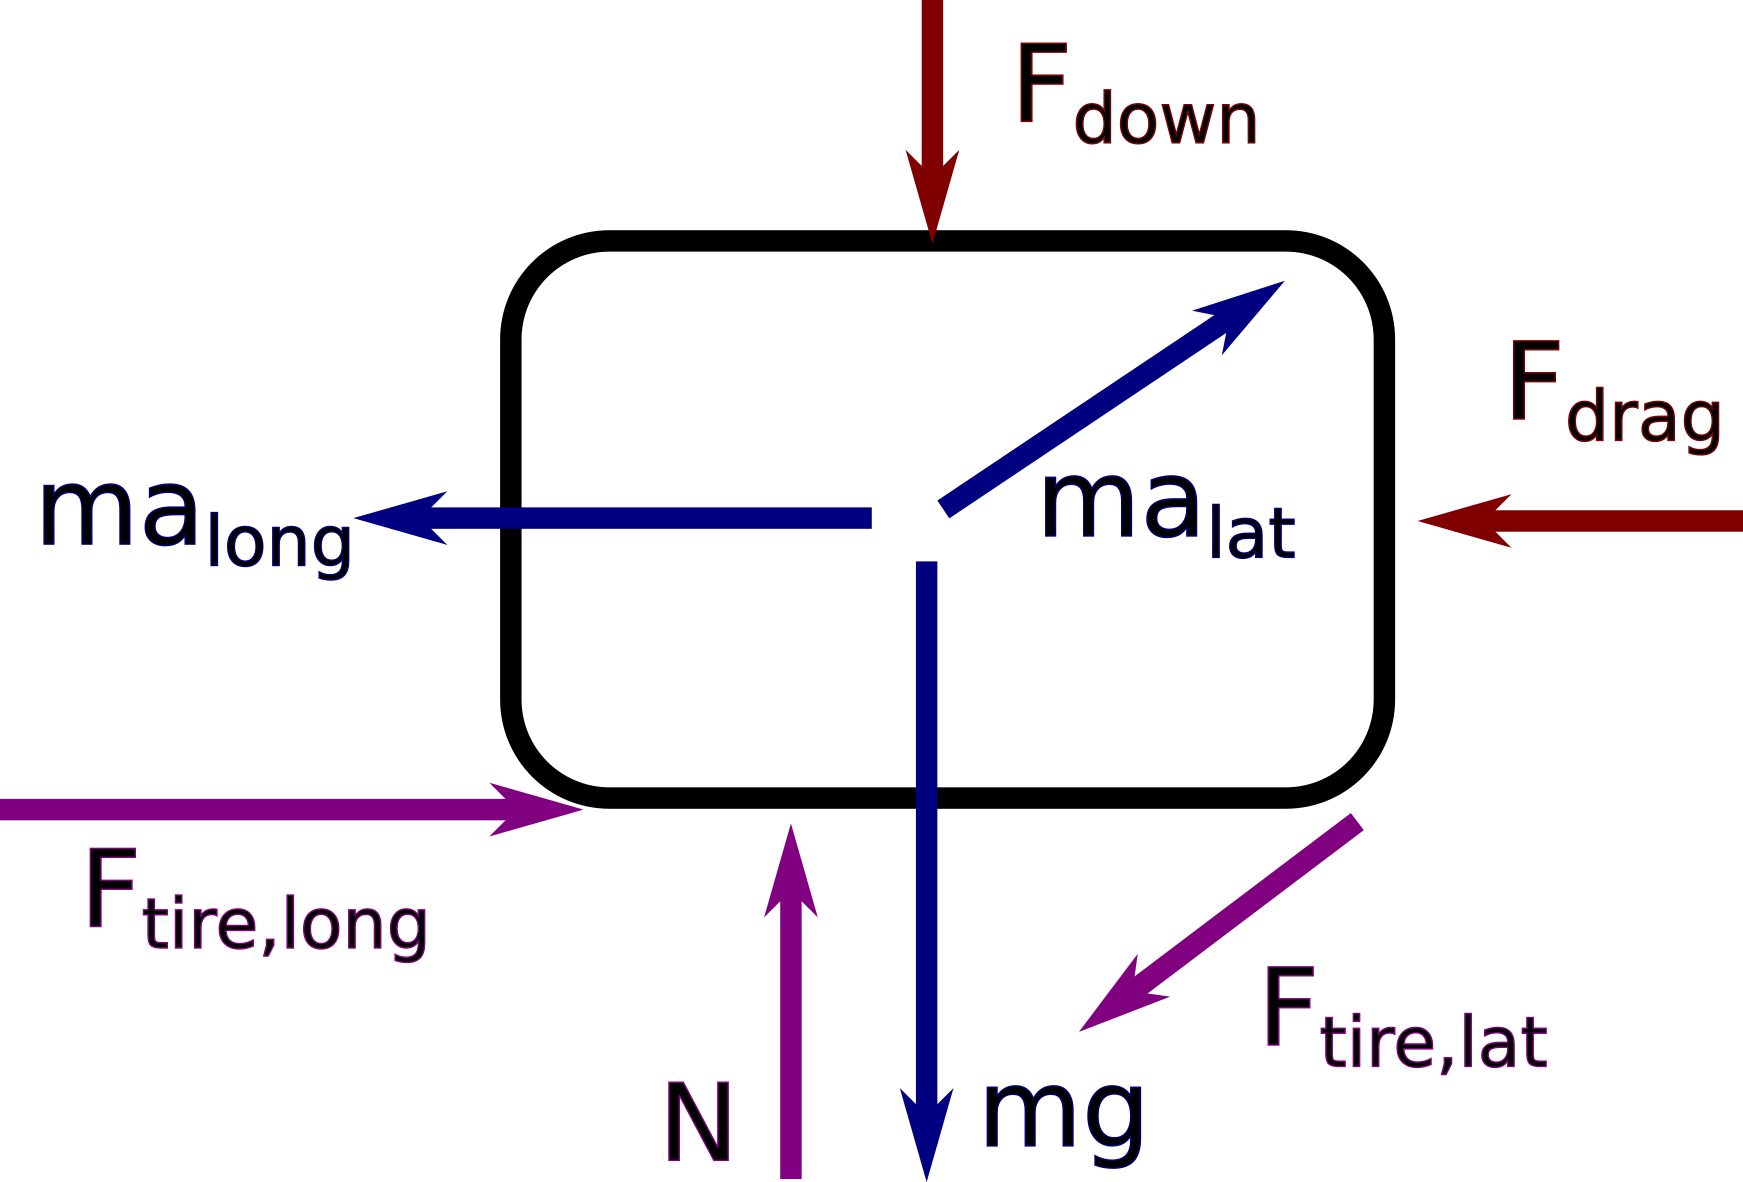
\includegraphics[width=0.4\textwidth]{single_fbd.png}
\end{center}

Now, we can begin the vehicle physics. The forces in the vertical direction, with no vertical acceleration (I.E. perfectly flat ground) are:

\begin{align}
	\Sigma F_z = m a_z \\
    -F_{down} -m g + N  = 0 \\
    N = m g + F_{down} \label{eq_z}
\end{align}

where $m$ is the vehicle mass, $g$ is the local acceleration due to gravity, and $N$ is the normal force of the track on the tires.

Given a specific vehicle path, we will prescribe a curvature the vehicle must pass through. The sum of forces in the lateral direction is, then,

\begin{align}
    \Sigma F_{lat} = m a_{lat} \\
    F_{tire,lat} = m v^2 k, \label{eq_lateral}
\end{align}

where $a_{lat}$ is lateral acceleration, $v$ is instantaneous vehicle velocity, and $k$ is curvature.

%By combining Equations \ref{eq_tire} and \ref{eq_lateral}, we can determine that the remaining longitudinal tire grip is:

%\begin{align}  
%    \Sigma F_{lateral} = m a_{lateral} \\
%    F_{tire,long,available} = \sqrt{ (\mu N)^2 - (m v^2 k)^2}, \label{eq_lateral}
%\end{align}
%
%Now, it is evident that we may not have remaining tire grip depending on velocity! As such, we will have to deal with going too fast later on- braking is a task that is not so straightforward.

The longitudinal forces acting on the vehicle are that of the tire and drag:

\begin{align}
	\Sigma F_{longitudinal} = m a_{longitudinal} \\
    a_{longitudinal} = \frac{\Sigma F_{longitudinal}}{m}\\
    a_{longitudinal} = \frac{F_{long,tire} - F_{drag} }{m} \label{eq_accel}
\end{align}

The force of the tire, though, can vary. In the case of braking, we assume the driver has the ability to lock up the tires, but does not; i.e., the tires apply all remaining grip: 
\begin{align}
F_{long,tire,braking} = -F_{tire,long,remaining}. \label{eq_accel_brake}
\end{align}

Acceleration, though, is more complicated, as the vehicle could be limited by either tire grip or engine power:

\begin{align}
	F_{long,tire,accel} = min(F_{tire,long,remaining}, F_{engine,limit})
\end{align}

We can now compute the overall acceleration of the vehicle and its final velocity.

\begin{align}
	a_{long} = \frac{F_{long,tire,...} - F_{drag}(v0)}{m} \\
	v_{final} = \sqrt{v_0^2 + 2 a_{long} d_{segment}}
\end{align}


\subsection{Code Implementation and Solver}

After creating a vehicle with known parameters and a track made of segments, the process of solving can begin. 

\subsubsection{Steps}

We will first examine a 'step'- how to get from the start state to end state of a given segment. The arguments for the 'step' function are as follows:

\begin{itemize}
\item \texttt{vehicle}: The vehicle and all its parameters
\item \texttt{prior\_result}: The simulation results from the previous step
\item \texttt{segment}: The current segment properties
\item \texttt{segment\_next}: The next segment's properties
\item \texttt{brake}: A flag indicating if braking is required
\item \texttt{shifting}: A flag indicating if the vehicle is currently shifting inbetween gears
\item \texttt{gear}: The current gear the vehicle is in
\end{itemize}

To begin, the final velocity and required accelerations, forces are calculated as described in the "Physics" section. If the tire grip is exceeded, an error is returned. The appropriate vehicle status is computed based on these values. To avoid oscillatory throttle-braking which also decreases cornering performance, a 'sustaining' strategy is utilized. If the vehicle is accelerating, running through a corner, and the prior status was braking, the next thing to do is sustain through the corner. If the vehicle was sustaining beforehand and curvature is relatively the same, continue to sustain. Sustaining is also triggered by running out of grip. Sustaining is simply solving for the steady-state velocity through a corner. Because of the nonlinearity of the equations, this is not a simple task. Something resembling bisection is employed. Luckily, the equations are simple enough that going faster will result in less remaining grip, and going slower will result in more.

Although this model does not allow for studying lateral load transfer, later ones do. To consistently study the effects of varying track, it is allowed to define an 'additional radius' that the vehicle is allotted to take a turn (if less track is provided, the radius is positive; if more track is used, the radius is negative).

\begin{align}
	k = \frac{k_{raw}}{1 + R_{additional} k_{raw}}
\end{align}

First, we will define remaining grip:

\begin{align}
	F_{long,remaining} = F_{long,remaining}(n_{tires} = 4, N = m g + F_{down}(v_f), F_{lat} = m v_f^2 k) - F_{drag}(v_f)
\end{align}

We will also determine the initial range of velocities we can use.

\begin{align}
	a_{max} = \frac{min(F_{engine},F_{tire,long,remaining})-F_{drag}}{m} \\
	a_{min} = \frac{-F_{tire,long,remaining}-F_{drag}}{m} \\
	v_{f,upper} = \sqrt{v_0^2 + 2 a_{max} d} \\
	v_{f,lower} = \sqrt{v_0^2 + 2 a_{min} d}
\end{align}

The bisection algorithm, from here, is fairly straightforward:

\begin{algorithm}[H]
\caption{Sustaining 'Bisection' Algorithm}
\begin{algorithmic}[1]
	\While{$excess < 0$ or $excess > \epsilon$}
		\State $v_f \gets \frac{v_{f,upper}+v_{f,lower}}{2}$
		\State $run$ $equations$ $of$ $motion$
		\If{$F_{long,remaining}(n_{tires},N,F_{lat}) - F_{drag}(v_{f}) < 0$}
			\State $v_{f,upper} \gets v_{f}$
		\Else
			\State $v_{f,lower} \gets v_{f}$
		\EndIf
	\EndWhile
\end{algorithmic}
\end{algorithm}

\subsubsection{Aerodynamic Strategy}

The aerodynamic strategy is also quite straightforward. Run a step with one aero configuration, and with another. If only one works, use that one. If both work, use the one with the better longitudinal acceleration. When braking, the choice is between 'full' or normal aero kit and an airbrake. When accelerating, the choice is between a DRS aero kit and the full aero kit.

\subsubsection{Overarching Solver}

With the strategy for determining the optimal (and feasible) acceleration around a corner determined, we can begin to determine the overall driving strategy to determine the optimal drive around a track.

Each iteration of the solver begins by taking a step based on the previous conditions. If this fails, the braking algorithm is initialized. A shifting algorithm is also employed. Stitching these pieces together and managing the edge conditions results in a rather large loop.

\subsubsection{Braking Algorithm}
The braking algorithm runs inside the main solver. The overall strategy is to 'replay' the part of the track leading up to the failure (loss of grip), but not so far back that time is spent sustaining before a corner. The strategy to do this has two main stages. The first is a 'scanning' phase, where large steps backwards are made to find, roughly, a window in which braking can initialize. the second is the 'bisection' phase, where a bisection algorithm is used to find the point of optimal performance.

\begin{algorithm}[H]
\caption{Braking Algorithm Pseudocode}
\begin{algorithmic}[1]
	\State Backup Output matrix (deep copy)
	\State $failure\_point \gets i$
	\State $lower\_brake\_bound \gets i-stepback\_amount$
	\State $upper\_brake\_bound \gets i$
	
	\While{True}
		\State $i = lower\_brake\_bound$
		\State Re-step from $i$, with \texttt{brake} on, til failure or $i > failure\_point$
		\If{failure}
			\State $lower\_brake\_bound \gets lower\_brake\_bound - stepback\_amount$
			\State $upper\_brake\_bound \gets upper\_brake\_bound - stepback\_amount$
		\Else
			\State Break out of loop
		\EndIf
	\EndWhile
	
	\While{$lower\_brake\_bound <= upper\_brake\_bound$}
		\State $i_{initial} = \frac{lower\_brake\_bound + upper\_brake\_bound}{2}$
		\State $i = i_{initial}$
		\State Re-step from $i$, with \texttt{brake} on, til failure or $i > failure\_point$
		\If{failure}
			\State $upper\_brake\_bound \gets i_{initial}$
		\Else
			\State $lower\_brake\_bound \gets i_{initial}$
		\EndIf
		\State Reset the Output matrix the the backup Output matrix from line 1
	\EndWhile
	
\end{algorithmic}
\end{algorithm}

\subsubsection{Shifting Algorithm}

Shifting seems like a simple matter of always keeping the transmission moving to the best gear. However, this ignores an issue presented by engines with ever-increasing power curves, and frictional forces that slow down the vehicle when not in gear. This slowing down of the vehicle means that by the time the next gear is ready, the gear that was previously selected is now the better gear. While we want to be in the best gear at all times, this marginal performance increase is obviously outweighed by the result that no power would be delivered to the wheels at any time.

To combat this problem, we simply dictate that the previous speed must be exceeded with the new gear before any further shifting is allowed. The pseudocode for this can be summarized as follows, and is triggered by the best gear (as measured by theoretical force at the tires at the current vehicle velocity) being different than the current gear.

\begin{algorithm}[H]
\caption{Shifting Algorithm Pseudocode}
\begin{algorithmic}[1]
	\State Compute $bestgear$
	\If{! \texttt{brake} and $bestgear \neq gear$ and $v > shift\_velocity$}
	\State $gear \gets gear + signof(bestgear - gear)$
	\State $shift\_velocity \gets v_i \times (1 + \epsilon)$
	\State $t_{shift} \gets t_i$
	\While{$t_i < t_{shift} + shift\_time$}
	\State Run steps like normal, but disable engine power by setting the \texttt{shifting} to on.
	\EndWhile
	\EndIf
\end{algorithmic}
\end{algorithm}

\section{Dual-Tire, Yaw-MOI Model}

\subsection{Physics}

A slight improvement can be made by accounting for the longitudinal load transfer induced by acceleration and heave of the vehicle, and yaw moment effects. This enables us to study the effect of center-of-gravity (CG) and center-of-pressure (CP) locations, as well as brake biasing, and any other parameter that would effect or be effected by longitudinal load transfer.

\begin{center}
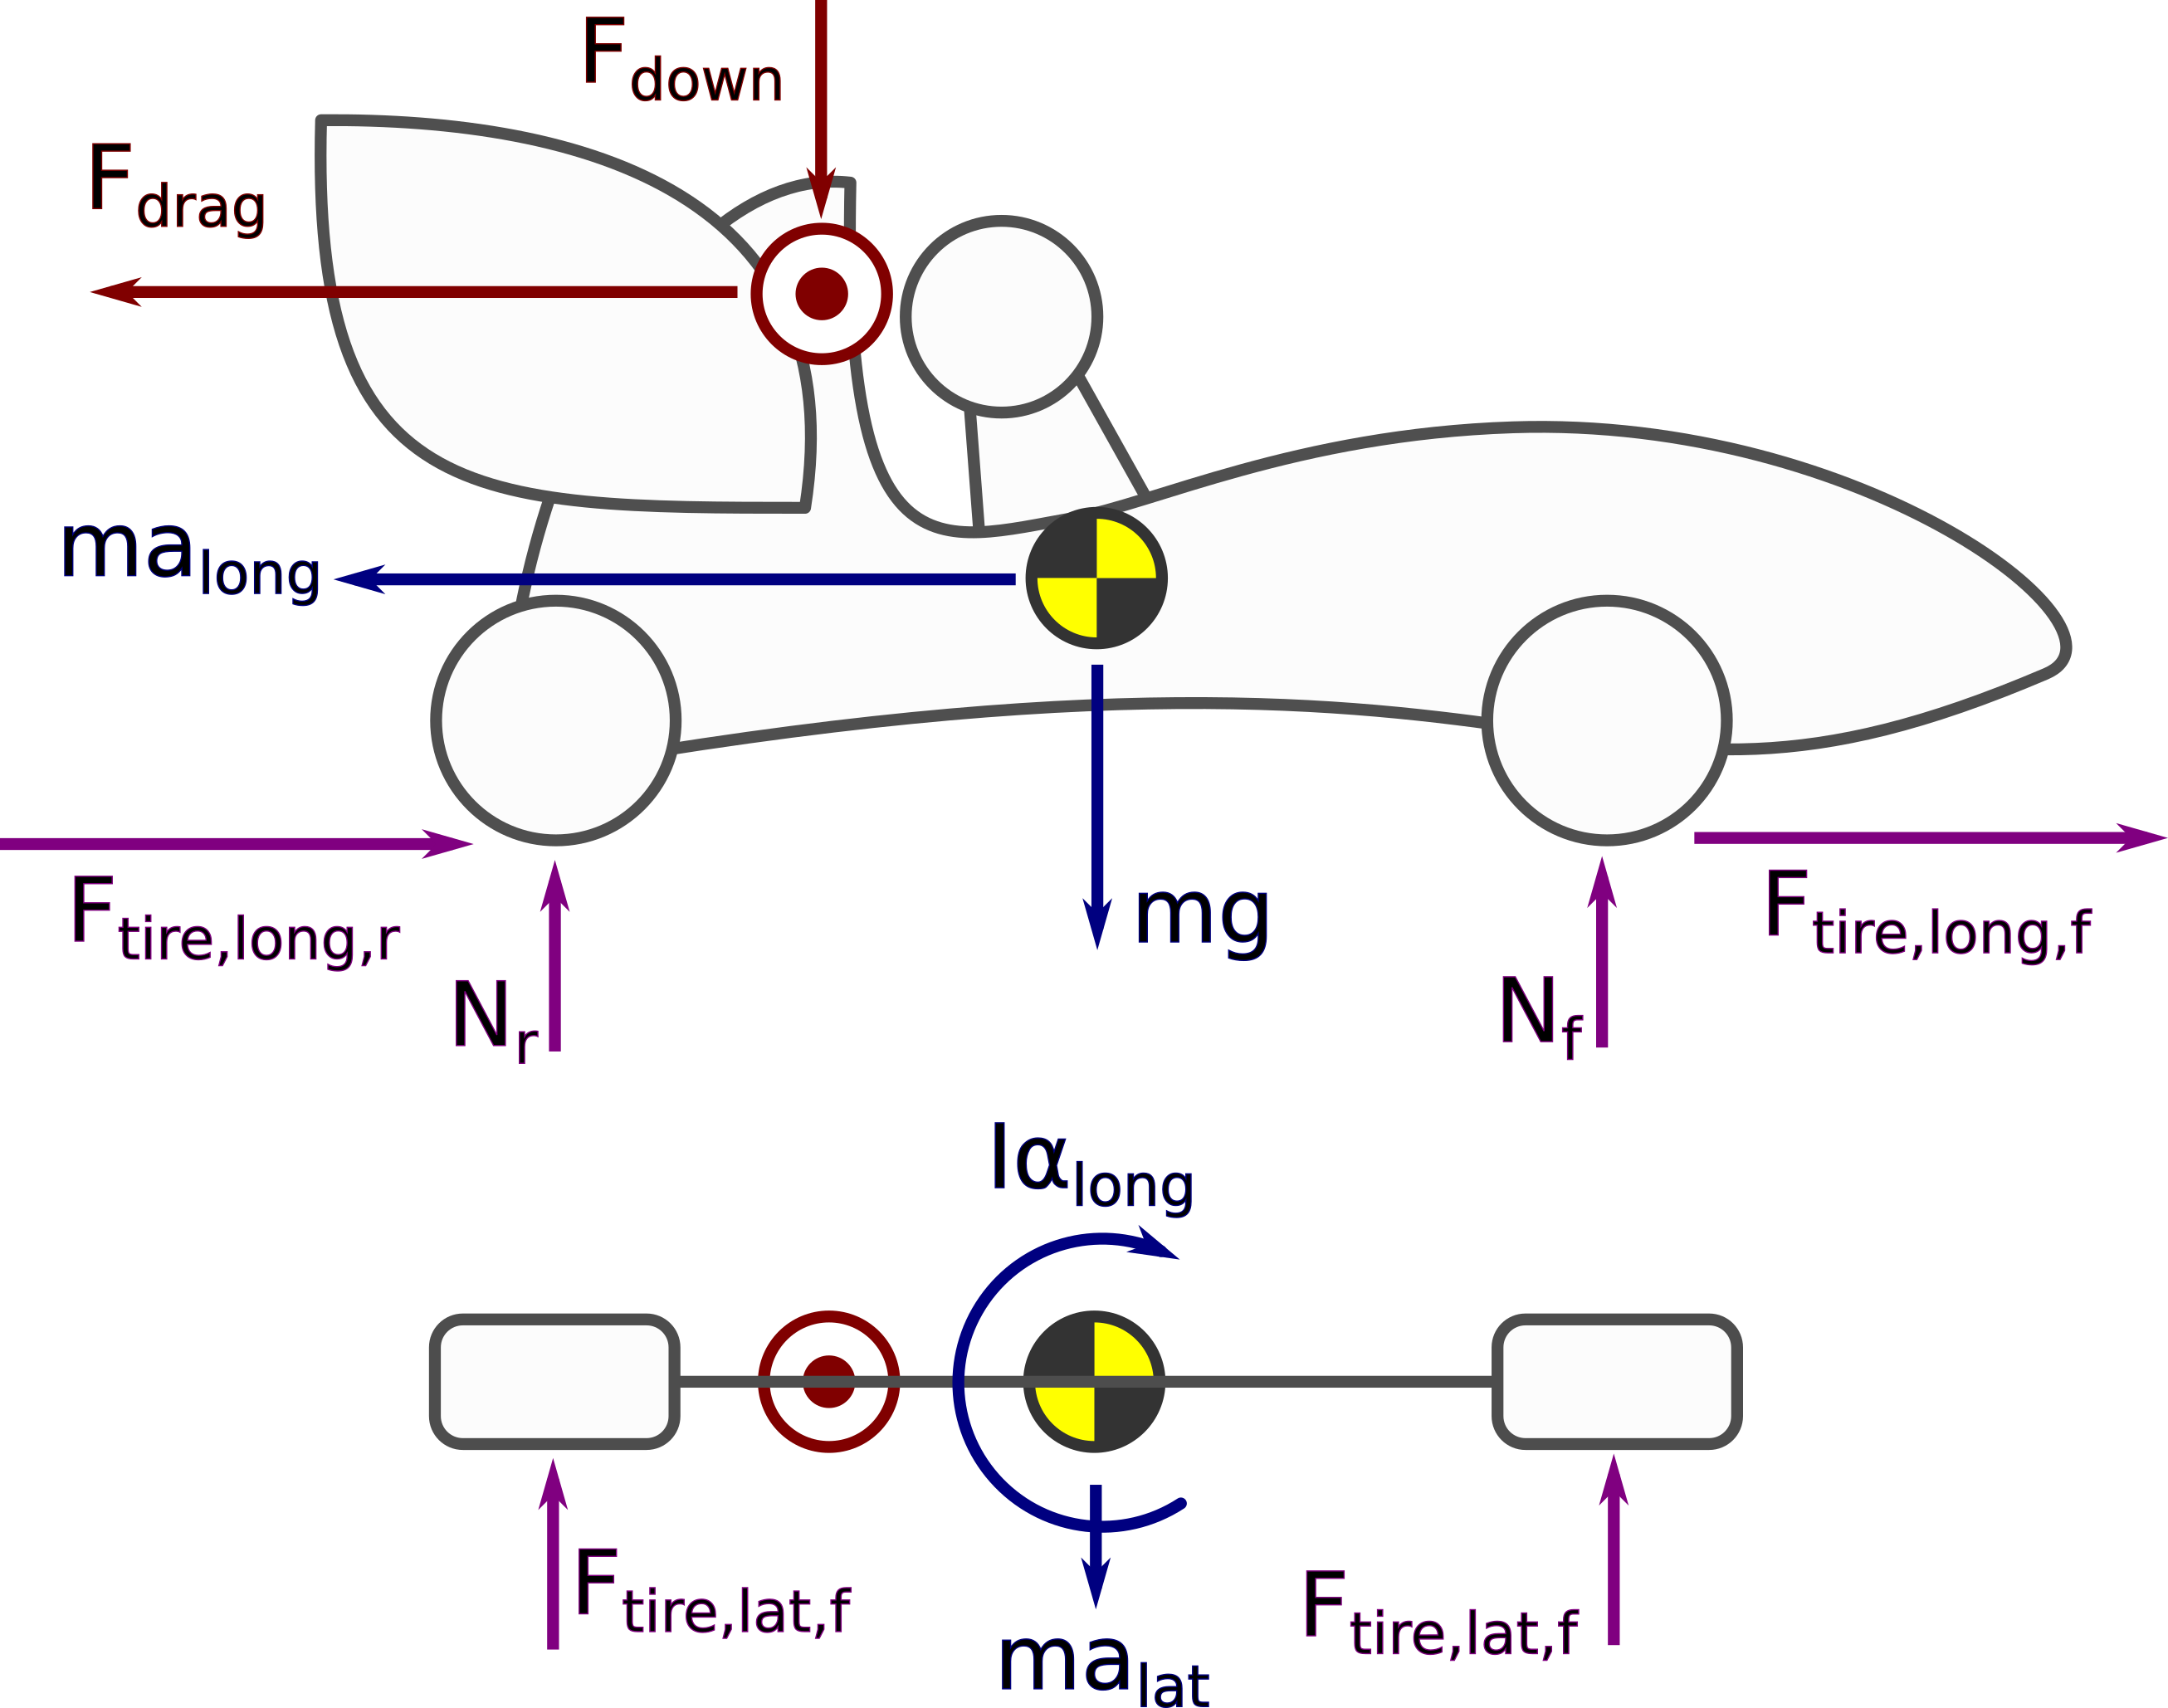
\includegraphics[width=\textwidth]{twotire_fbd.png}
\end{center}

The vehicle physics begin with the summation of forces and moments in the vertical, longitudinal, and lateral directions.

\begin{align}
	\Sigma F_{vert} = m a_{vert} \\
	\Sigma F_{lat} = m a_{lat} \\
	\Sigma F_{long} = m a_{long} \\
	\Sigma M_{vert} = \Sigma m a \times r + I_{yaw} \alpha \\
	\Sigma M_{lat} = \Sigma m a \times r + I_{yaw} \alpha \\
\end{align}

\begin{align}	
	\Sigma F_{vert} = N_{f} + N_{r} - m g - F_{down}(v_0) = 0 \\
	\Sigma F_{lat}  = F_{tire,lat,f} + F_{tire,lat,f} = m a_{lat} = m v^2 k \\
	\Sigma F_{long} = F_{tire,long,f} + F_{tire,long,f} - F_{drag}(v_0) = m a_{long} \\	
	\Sigma M_{vert} = F_{tire,lat,f} l_{wheelbase} = m v^2 k l_{CG} + I_{yaw} \alpha \\
	\Sigma M_{lat}  = N_{f} l_{wheelbase} + F_{drag}(v_0) h_{CP} - F_{down}(v_0) l_{CP} - m g l_{CG} = m a_{long} h_{CG}
\end{align}

where subscripts $f$ denote relation to the front tires, and $r$ denote relation to the rear tires. $l{CG}$ and $l_{CP}$ are the longitudinal distance from the rear tires to the CG and CP, respectively. $h_{CG}$ and $h_{CP}$ are the vertical height from the ground to the CG and CP, respectively. $l_{wheelbase}$ is the distance from the rear to front tires. $I_{yaw}$ is the moment of inertia about the vertical axis passing through the CG. $\alpha$ is the yaw acceleration, which is computed as:

\begin{align}
	\omega = \frac{v}{r} = v k \\
	\alpha = \frac{\D \omega}{\D t} = v \frac{\D k}{\D t} + k \frac{\D v}{\D t} \\
	\alpha = v \frac{\D k}{\D x} \frac{\D x}{\D t} + k a_{long} \\
	\alpha = v^2 \frac{k_f - k_0}{\Delta x} + k_0 a_{long}
\end{align}

It should be noted that the summation of forces about the longitudinal axis results in the inertial force of the vehicle being the only thing to produce a moment, and as such, this is ignored, understanding that lateral load transfer is not modeled by this set of equations.

Solution of this is somewhat ugly, and most importantly, cannot be done explicitly. As such, the solution is attempted at first in a marginal fashion; this will be discussed later.

\subsubsection{The Marginal Physics}
This method begins by computing the required lateral force for each tire. $N_f, N_r, v0$ are presumed to be known from the previous iteration.

\begin{align}
	F_{tire,lat,f} = \frac{l_{CG}}{l_{wheelbase}} m v^2 k + \frac{\alpha I_{yaw}}{l_{wheelbase}}  \\ 
	F_{tire,lat,r} = (1-\frac{l_{CG}}{l_{wheelbase}}) m v^2 k - \frac{\alpha I_{yaw}}{l_{wheelbase}}
\end{align}

The remaining longitudinal forces $F_{tire,remaining,long}$ are computed as discussed previously (normal forces are presumed to be known). 

Two models of braking may be employed: perfect brake biasing, and fixed brake biasing. Perfect brake biasing is simple; just use all available grip to decelerate:

\begin{align}
	F_{tire,long,f} = -F_{tire,remaining,long,f} \\
	F_{tire,long,r} = -F_{tire,remaining,long,r}
\end{align}

Fixed brake biasing is less so. First, the maximum total braking force must be found:

\begin{align}
	F_{brake} = min(\frac{F_{tire,remaining,long,f}}{X_{f}}, \frac{F_{tire,remaining,long,r}}{X_{r}}),
\end{align}

where $X$ is the brake bias for the front or rear tires ($X_f + X_r = 1$). Then, the brake force can be applied to the front and rear tires in the corresponding amount:

\begin{align}
	F_{tire,long,f} = - F_{brake} X_{f} \\
	F_{tire,long,r} = - F_{brake} X_{r}
\end{align}

Acceleration is the same as the point-mass model, but it is important to note that the rear-wheel tires are considered; assuming RWD rather than FWD or AWD. The overall longitudinal force, longitudinal acceleration, and final velocity can then be computed.

\begin{align}
	\Sigma F_{longitudinal} = F_{tire,long,f} + F_{tire,long,r} - F_{drag}(v_0) \\
	a_{long} = \frac{ F_{tire,long,f} + F_{tire,long,r} - F_{drag}(v_0)}{m} \\
	v_{final} = \sqrt{v_0^2 + 2 a_{long} d_{segment}}
\end{align}

The normal force is computed for the next iteration, and for checks.

\begin{align}
	N_f = (1 - \frac{l_{CG}}{l_{wheelbase}}) m g 
			+ (1 - \frac{l_{CP}}{l_{wheelbase}}) F_{down}
			- m a_{long} \frac{h_{CG}}{l_{wheelbase}} 
			- \frac{h_{CP}}{l_{wheelbase}} F_{drag} \\
	N_r = \frac{l_{CG}}{l_{wheelbase}} m g 
			+ \frac{l_{CP}}{l_{wheelbase}} F_{down}
			+ m a_{long} \frac{h_{CG}}{l_{wheelbase}} 
			+ \frac{h_{CP}}{l_{wheelbase}} F_{drag}
\end{align}

\subsubsection{Working Backwards}
This method determines the forces on the vehicle given a prescribed $a_{long}$.

The normal forces on the tires can be found by solving the summation of forces in the and vertical direction, and summation of moments about the lateral axis. This results in:

\begin{align}
	N_f = (1 - \frac{l_{CG}}{l_{wheelbase}}) m g 
			+ (1 - \frac{l_{CP}}{l_{wheelbase}}) F_{down}
			- m a_{long} \frac{h_{CG}}{l_{wheelbase}} 
			- \frac{h_{CP}}{l_{wheelbase}} F_{drag} \\
	N_r = \frac{l_{CG}}{l_{wheelbase}} m g 
			+ \frac{l_{CP}}{l_{wheelbase}} F_{down}
			+ m a_{long} \frac{h_{CG}}{l_{wheelbase}} 
			+ \frac{h_{CP}}{l_{wheelbase}} F_{drag}
\end{align}

The required lateral forces from the tires are also computed:

\begin{align}
	F_{tire,lat,f} = \frac{l_{CG}}{l_{wheelbase}} m v^2 k + \frac{\alpha I_{yaw}}{l_{wheelbase}}  \\ 
	F_{tire,lat,r} = (1-\frac{l_{CG}}{l_{wheelbase}}) m v^2 k - \frac{\alpha I_{yaw}}{l_{wheelbase}}
\end{align}

From here, the required longitudinal tire grip can be computed.
\begin{align}
	F_{tire,long,total,required} = \frac{a_{long}}{m} + F_{drag}(v)
\end{align}

We must then compute the required longitudinal tire grip to maintain the desired $a_{long}$ and counteract drag. For the acceleration case, this is straightforward:

\begin{align}
	F_{tire,long,r,required} = F_{tire,long,total,required}
\end{align}

For the braking case where fixed biasing is used, the process is very simple: distribute the required force between the tires.
\begin{align}
	F_{tire,long,r,required} = F_{tire,long,total,required} X_r \\
	F_{tire,long,f,required} = F_{tire,long,total,required} X_f
\end{align}

For the braking case where perfect biasing is used, this requires some thinking. Since in this model, the front and rear braking forces are colinear, it makes no difference to where the braking force is distributed (provided that the maximum grip is not exceeded). We will use up all of the more-available tire's grip before using the less-available tire's grip.

\begin{algorithm}[H]
\caption{Perfect Biasing Braking Algorithm}
\begin{algorithmic}[1]
	\State $F_{tire,long,more,required}$ = $F_{tire,long,total,required}$
	\If{$F_{tire,long,remaining,more} < F_{tire,long,more,required}$}
	\State	$F_{tire,long,remaining,less}$ = $F_{tire,long,total,required}$ - $F_{tire,long,more,required}$
	\EndIf
\end{algorithmic}
\end{algorithm}

From here, checks may be performed to ensure that grip is used appropriately, and final velocity is calculated much like before.



\subsection{Code Implementation and Solver}

\subsubsection{Take A Step}

Taking a step is significantly more complicated in the two-tire model, because acceleration induces longitudinal load transfer. As mentioned before, it is difficult to solve the equations of motion. More complex checks must be employed. The equations described in "The Marginal Physics" are employed at first. After this, the remaining longitudinal grip is evaluated at the new vehicle velocity, and the next segment's curvature. If there is not sufficient grip on either of the tires, then we will need to iteratively solve for an acceleration that will work and still be optimal.

To solve for an acceleration that will work and still be optimal, a simple loop is employed to scan over a range of vehicle velocities (which are the same as the bounds for bisection used in the point-mass model). The physics discussed in the "Working Backwards" section are employed to check. This was intended to be bisection at first, as this would enable more precision. How to make this work was not immediately self-evident though, but Thad does have some ideas on how to make it work. As it stands, the range of possible vehicle velocities is swept through, and then the 'best' (highest amplitude of acceleration, depending on if braking is desired) velocity is chosen.

\subsubsection{Putting it Together}

The overall solver for the two-tire model is identical to the point-mass model, save for the braking algorithm employed. The braking algorithm employed here does not use the bisection stage, but uses smaller steps backwards. This was done because of solution stability. Bisection is the ideal algorithm, but stability issues meant having to forgo the computational efficiency of the bisection algorithm.

\section{Point Simulations}

Once multiple lap time simulations have been ran, the next important thing to do is put the pieces together and simulate points at a competition.

The points scored at each event can be found from the FSAE rulebook:

\begin{align}
	P_{acceleration} = 95.5 \frac{1.5 t_{best}}{0.5 (t_{acceleration} - 1)} + 4.5 \\
	P_{skidpad} = 71.5 \frac{\frac{1.45 t_{best}}{t_{skidpad}}^2 -1}{1.45^2 - 1} + 3.5 \\
	P_{autocross} = 118.5 \frac{1.45 t_{best}}{0.45 (t_{autocross} - 1)} + 6.5 \\
	P_{endurance} = 250 \frac{1.45 t_{best}}{0.45 (t_{endurance} - 1)} + 25
\end{align}

Efficiency score calculation is more complex.

\begin{align}
	EF_i = \frac{t_{best}}{t_{endurance}} \frac{CO2_{best}}{CO2_{endurance}} \\
	P_{efficiency} = 100 \frac{\frac{EF_{min}}{EF_i}-1}{\frac{EF_{min}}{EF_{max}}-1}
\end{align}

Lap times, best times at previous tracks, and estimated CO2 production can simply be plugged into these formulae. Estimation of the CO2 production, hopefully, is good enough.

\section{Four-Tire, Yaw-MOI Model}

This model is mostly a tweak of the two-tire model, so the physics changes only will be discussed here.

\subsection{Physics}

Adding four tires to the chassis is fairly simple from this point. We consider the chassis and suspension as a torsional spring assembly as shown below:

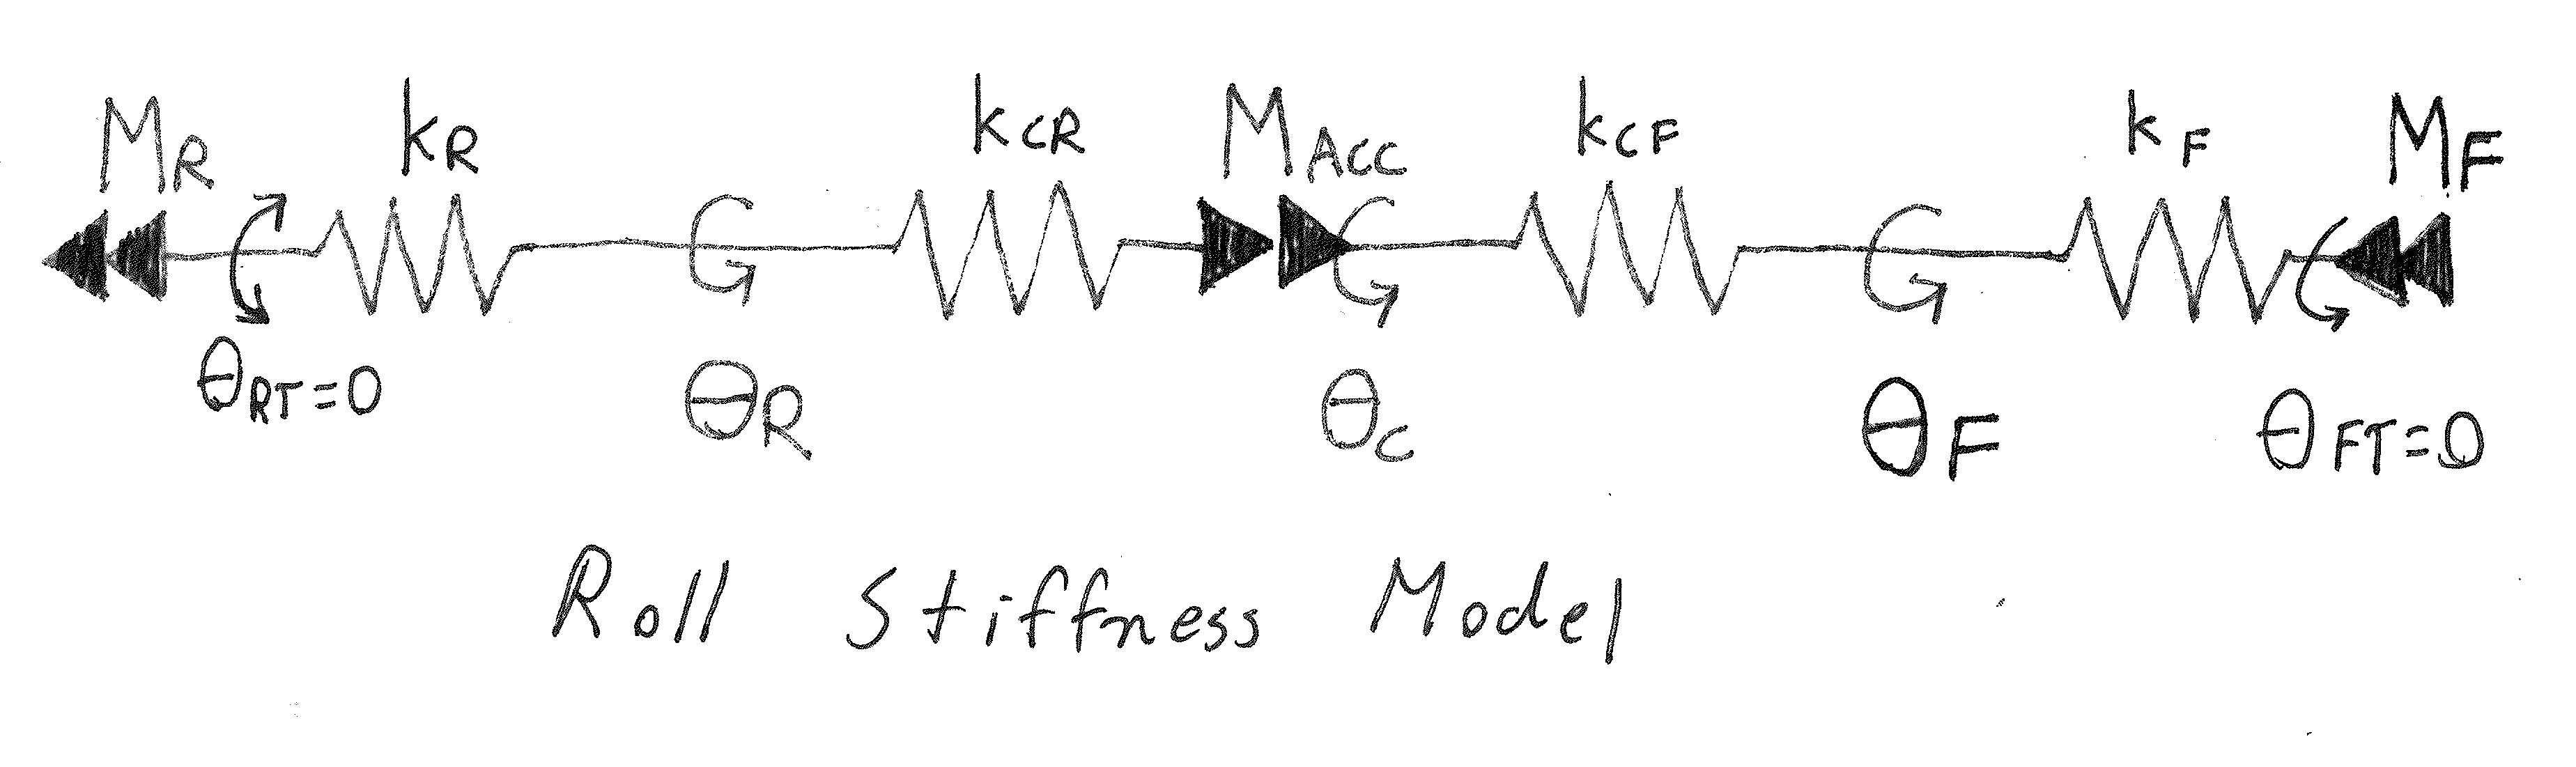
\includegraphics{tors_springs.png}

where:
\begin{itemize}
\item $M_r$ and $M_f$ are the moments by the rear and front tires
\item $M_f$ is the moment produced by the front tires
\item $M_{acc}$ is the moment produced by lateral acceleration
\item $k_f$ and $k_r$ is the suspension roll stiffness for front and rear
\item $\theta_f$, $theta_r$, and $theta_c$ is the vehicle roll at the front and rear suspension points, and CG
\end{itemize}

We can write the following spring equations:

\begin{align}
	k_r \theta_r = M_r \\
	k_f \theta_f = M_f \\
	k_cr (\theta_c-\theta_r) = M_r \\
	k_cf (\theta_c-\theta_f) = M_f
\end{align}

Including the torque balance equation leaves us with 5 equations and 5 unknowns ($M_r$, $M_f$, and $\theta$'s):
\begin{align}
	M_{acc} = M_r + M_f
\end{align}

Solving these equations yields:

\begin{align}
	M_f = M_{acc} k_{cf} k_f \frac{k_{cr}+k_r}{k_{cf} k_{cr} k_f+k_{cf} k_{cr} k_r+k_{cf} k_f k_r+k_{cr} k_f k_r}\\
    M_r = M_{acc} k_{cr} k_r \frac{k_{cf}+k_f}{k_{cf} k_{cr} k_f+k_{cf} k_{cr} k_r+k_{cf} k_f k_r+k_{cr} k_f k_r}
\end{align}

Generally, $k_r$, $k_f$ are roughly known, but $k_cr$ and $k_cf$ are not- but overall chassis $k_c$ stiffness is. We will approximate the chassis as having linearly distributed stiffness. This gives us:

\begin{align}
	k_cr = \frac{k_c}{\frac{l_{CG}}{l_{wheelbase}}}\\
	k_cf = \frac{k_c}{1 - \frac{l_{CG}}{l_{wheelbase}}}
\end{align}

It is important to note that this assumes that the ground is flat, and assumes steady state (that us, no dampers nor roll acceleration).

If we know the forces on the front tires and on the rear tires $N_f$ and $N_r$ we can compute the normal force on each tire. Inside tires have subscript 1, outside subscript 2.

\begin{align}
	N_{f,1} = \frac{N_{f}}{2} - \frac{M_f}{w_f} \\
	N_{f,2} = \frac{N_{f}}{2} + \frac{M_f}{w_f} \\
	N_{r,1} = \frac{N_{r}}{2} - \frac{M_r}{w_r} \\
	N_{r,2} = \frac{N_{r}}{2} + \frac{M_r}{w_r}
\end{align}

Currently, the tire lateral grips are distributed between tires to try and equalize the longitudinal grip. If this is not possible (i.e. one tire has immense grip), the lateral load is taken completely by the better-loaded tire, and the maximum tire grip for each tire is assumed to be that of the lower one. This enforces the assumption of 50/50 left-right brake bias (a good assumption) and an open differential (a poor assumption).

% \section{Post-Processing}

% Evë please write something, thanks.

% \section{Future Plans}

% RoseLap 

\section{Appendix}

\lstinputlisting[basicstyle=\small,caption={Example Vehicle Definition File},label=vehicle_start_here]{params/vehicles/VEHICLE_START_HERE.yaml}

\end{document}
